\documentclass[12pt,titlepage]{scrreprt}
\usepackage[ngerman]{babel}
\usepackage[utf8]{inputenc}
\usepackage{color}
\usepackage{float}
\usepackage[a4paper,lmargin={2.5cm},rmargin={2.5cm},tmargin={2.5cm},bmargin = {2cm}]{geometry}
\usepackage{amssymb}
\usepackage{amsthm}
\usepackage{graphicx}
\usepackage{subfig}
\usepackage{wrapfig}
\usepackage{url}
\usepackage{cite}


\begin{document}
% % Activate the following line by filling in the right side. If for example the name of the root file is Main.tex, write
% "...root = Main.tex" if the chapter file is in the same directory, and "...root = ../Main.tex" if the chapter is in a subdirectory.
 
%!TEX root =  TNTinderSee.tex

% mehrere Bilder in einer Bildumgebung mit 
%\subfloat{bild.jpg}


\begin{titlepage}
\thispagestyle{empty}
 \begin{center}
 \begin{figure}[htbp]
    \centering
 %   \subfloat{\includegraphics[width=0.15\textwidth]{Bilder/Titel/bild-firma.JPG}}\quad
   %  \subfloat{\includegraphics[width=0.25\textwidth]{Bilder/Titel/bild-uni 
%oder fh.JPG}}
\end{figure}
\vspace*{1cm}
 \Large{Schiller-Gymnasium Offenburg }

  \vspace*{1.5cm}
 {\huge Thema}
 \vspace*{1cm} \\
 {\Large Abschlussbereicht\\von\\Eitel, Martin \\ \texttt{marjelly1@gmail.com}\\Komyakov, Alexander \\\texttt{alexander.komyakov@lynxisgod.eu} \\ Rehwinkel, Antonio \\ \texttt{antonio.rehwinkel@schiller-og.de} \\ Sauerbrey, Luisa \\ \texttt{luisa.sauerbrey@schiller-og.de}
 \vspace{0.5cm}
 {\Large \bfseries \\}
 \vspace{0.5cm}
 {\Large geboren am dein Geburtstag}
 \vfill
  \vspace*{1.5cm}
\begin{table}[h]
	\centering
	\begin{tabular}{|l| l|}\hline
		Aufgabensteller & Prof. \\ \hline
		Durchgeführt bei: & Firmenname\\ \hline
		Betreuer: & Betreuer Firma\\ Marek Czernohous \\ \hline
		Wissenschaftspate & \\ Prof. Dr. Jens Greinert\\ \hline
		Arbeit vorgelegt am: & Datum\\ \hline
	\end{tabular}
\end{table}
}
\end{center}
\end{titlepage}


\begin{titlepage}

	

\title{Die Auswirkung von Munitionshalden auf die Wasserqualität der Ostsee zwischen Vilm und Lauterbach}
\subtitle{Ausfahrt vom 18.07. - 21.07.2021}
\titlehead{\centering\includegraphics[width=15cm]{Bilder/DSC05220}}


\author{Eitel, Martin; Komyakov, Alexander; \\ Rehwinkel, Antonio; Sauerbrey, Luisa\\ \and Schiller-Gymnasium Offenburg}

\publishers{Wissenschaftspate: Prof Dr. Jens Greinert \texttt{jgreinert@geomar.de} \\
\vspace*{2ex} Betreuer: Marek Czernohous \texttt{m.czernohous@schiller-offenburg.de}}
%- \\ Schiller-Gymnasium Offenburg}

\maketitle

\end{titlepage}
\addchap{Kurzfassung}
Unser Wettbewerbsbeitrag umfasst

\tableofcontents
% Activate the following line by filling in the right side. If for example the name of the root file is Main.tex, write
% "...root = Main.tex" if the chapter file is in the same directory, and "...root = ../Main.tex" if the chapter is in a subdirectory.
 
%!TEX root =  TNTinderSee.tex

\chapter[Einleitung]{Einleitung}

Im Meer lagernde Munition stellt eine Gefahr dar. Nicht unbedingt durch unmittelbare Detonotationsgefahr, 
sondern durch die langsame Zersetzung, die die enthaltenen Sprengstoffe nach und nach 
freilegt\cite{zeitbomben}. Die Entstehung sprengstofftypischer Abbauprodukte, sowie das direkte Austreten 
giftiger Stoffe, stellen Gesundheitsgefährung exponierter Meerestiere, aber auch Menschen dar, denn die
Abbauprodukte gelten als krebserregend und das potentiell austretende Phosphor lagert sich an den Stränden 
ab und ist von Bernstein kaum zu unterscheiden. Als wir den Meereswettbewerb mit der Aldebaran fanden, 
fühlten wir uns gezwungen nachzuforschen wie groß die Gefahr schon heutzutage ist.\\

Wir wollten in einem potentiellem Munitionsabwurfsgebiet messen, wie groß die Anteile der Schadstoffe sind und 
ob noch etwas von den Granaten und Bomben zu sehen ist. Dazu entschieden wir uns für ein Gebiet kurz Vilm,
da hier angeblich zwei Schuten nach dem Zweiten Weltkrieg mit Munition beladen explodiert sein sollen.\\

Das Naturschutzgebiet Vilm liegt in etwa 100 Meter Entfernung zu der Explosionsstelle und auch weiter 
entfernte Orte können durch Ablagerungen und Schadstoffe in Fisch-Fängen betroffen sein.\\

In Zusammenarbeit mit der Aldebaran und dem Geomar wollten wir die Wracks kartieren und die Schadstoffwerte in
der direkten Umgebung messen. Besonders interessant wäre die beförderte Munition gewesen. Die Frage der
Ortung und Untersuchung der möglichen Funde konnten wir zusammen mit dem Geomar lösen. Mithilfe eines 
"Multibeams" sollten wir interessante Orte ohne Tauchgang finden können um später mit dem Schuleigenen 
ROV die Orte genauer unter die Lupe nehmen zu können. Auch Sedimentproben dirket neben den Fundstätten 
konnten wir mithilfe eines eignene Aufsatzes realisieren.\\

Wir befürchteten hohe Werte für Phosphor und sprengstofftypische Verbindungen wie Trinitrotoluol (TNT) 
zu messen und unter Umständen sogar Granaten oder Bomben zu finden. Falls dies passieren sollte, würde 
sich für uns die Frage stellen, wie sich diese Munition auf die Öknomie ausgewirkt hat. \\

In schon existierenden Forschungen zeigt sich, 
https://www.schleswig-holstein.de/DE/UXO/EN/Themes/Subjects/assessements.html

https://www.geomar.de/fileadmin/content/service/presse/Pressemitteilungen/2020/pm_2020_37_munition-sh.pdf

https://www.eskp.de/schadstoffe/wie-weiter-mit-den-kampfmittelaltlasten-im-meer-9351103/

https://www.eskp.de/schadstoffe/wie-weiter-mit-den-kampfmittelaltlasten-im-meer-9351103/

Themenfindung, Relevanz, entscheidende Fragen, Lösungsansätze, Forschungsstand mit Quellen, Erwartungen, konkrete Fragen.

% Activate the following line by filling in the right side. If for example the name of the root file is Main.tex, write
% "...root = Main.tex" if the chapter file is in the same directory, and "...root = ../Main.tex" if the chapter is in a subdirectory.
 
%!TEX root =  TMTinderSee.tex

\chapter[Hauptteil]{Hauptteil}

\section{Versuchsplanung}
Oh dear, hier muss noch was rein!


\subsection{Kartierung}
    Alle Kartierungsvorgänge wurden mit der Free Open Source Software\\
\emph{QGIS}\cite{qgis}durchgeführt.
\begin{figure}[ht]
    \centering
    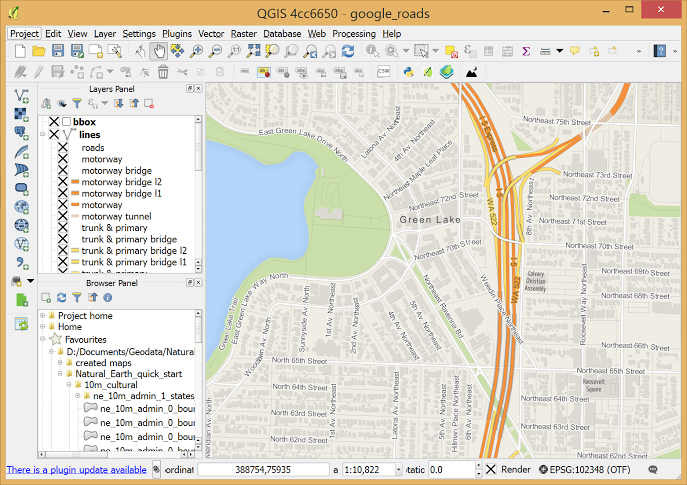
\includegraphics[width=.4\linewidth]{Bilder/QGIS/about-screenshot.png}
    \caption[fig:qgisabout]{QGIS-Benutzeroberfläche}
\end{figure}
\\Mithilfe dieser Software lassen sich basierend auf bereits existierenden Karten, 
wie beispielsweise \emph{OpenStreetMap}\cite{ostrm} oder \emph{OpenSeaMap}\cite{oseam},
eigene Routen und Points of \\Interest(POIs) ohne großen Aufwand eintragen. Genauso 
leicht erfolgt der Import sowie vom Multibeam,  als auch von den Navigationsgeräten 
der ALDEBARAN gespeicherten Positions- und Geschwindigkeitsdaten.\\


Basierend auf dem QGIS-Projekt von \jens, welches die \emph{OpenStreetMap}, sowie den Munitionslagerstättendaten von den Webseiten
\emph{AmuCad}\cite{amucad} und \emph{Munition im Meer}\cite{muninmeer}
als Basis benutzt, konnten wir unsere Route planen (vgl. Abbildungen \ref{fig:route} und \ref{fig:multibeam_route}).

\begin{figure}[]
    \centering
    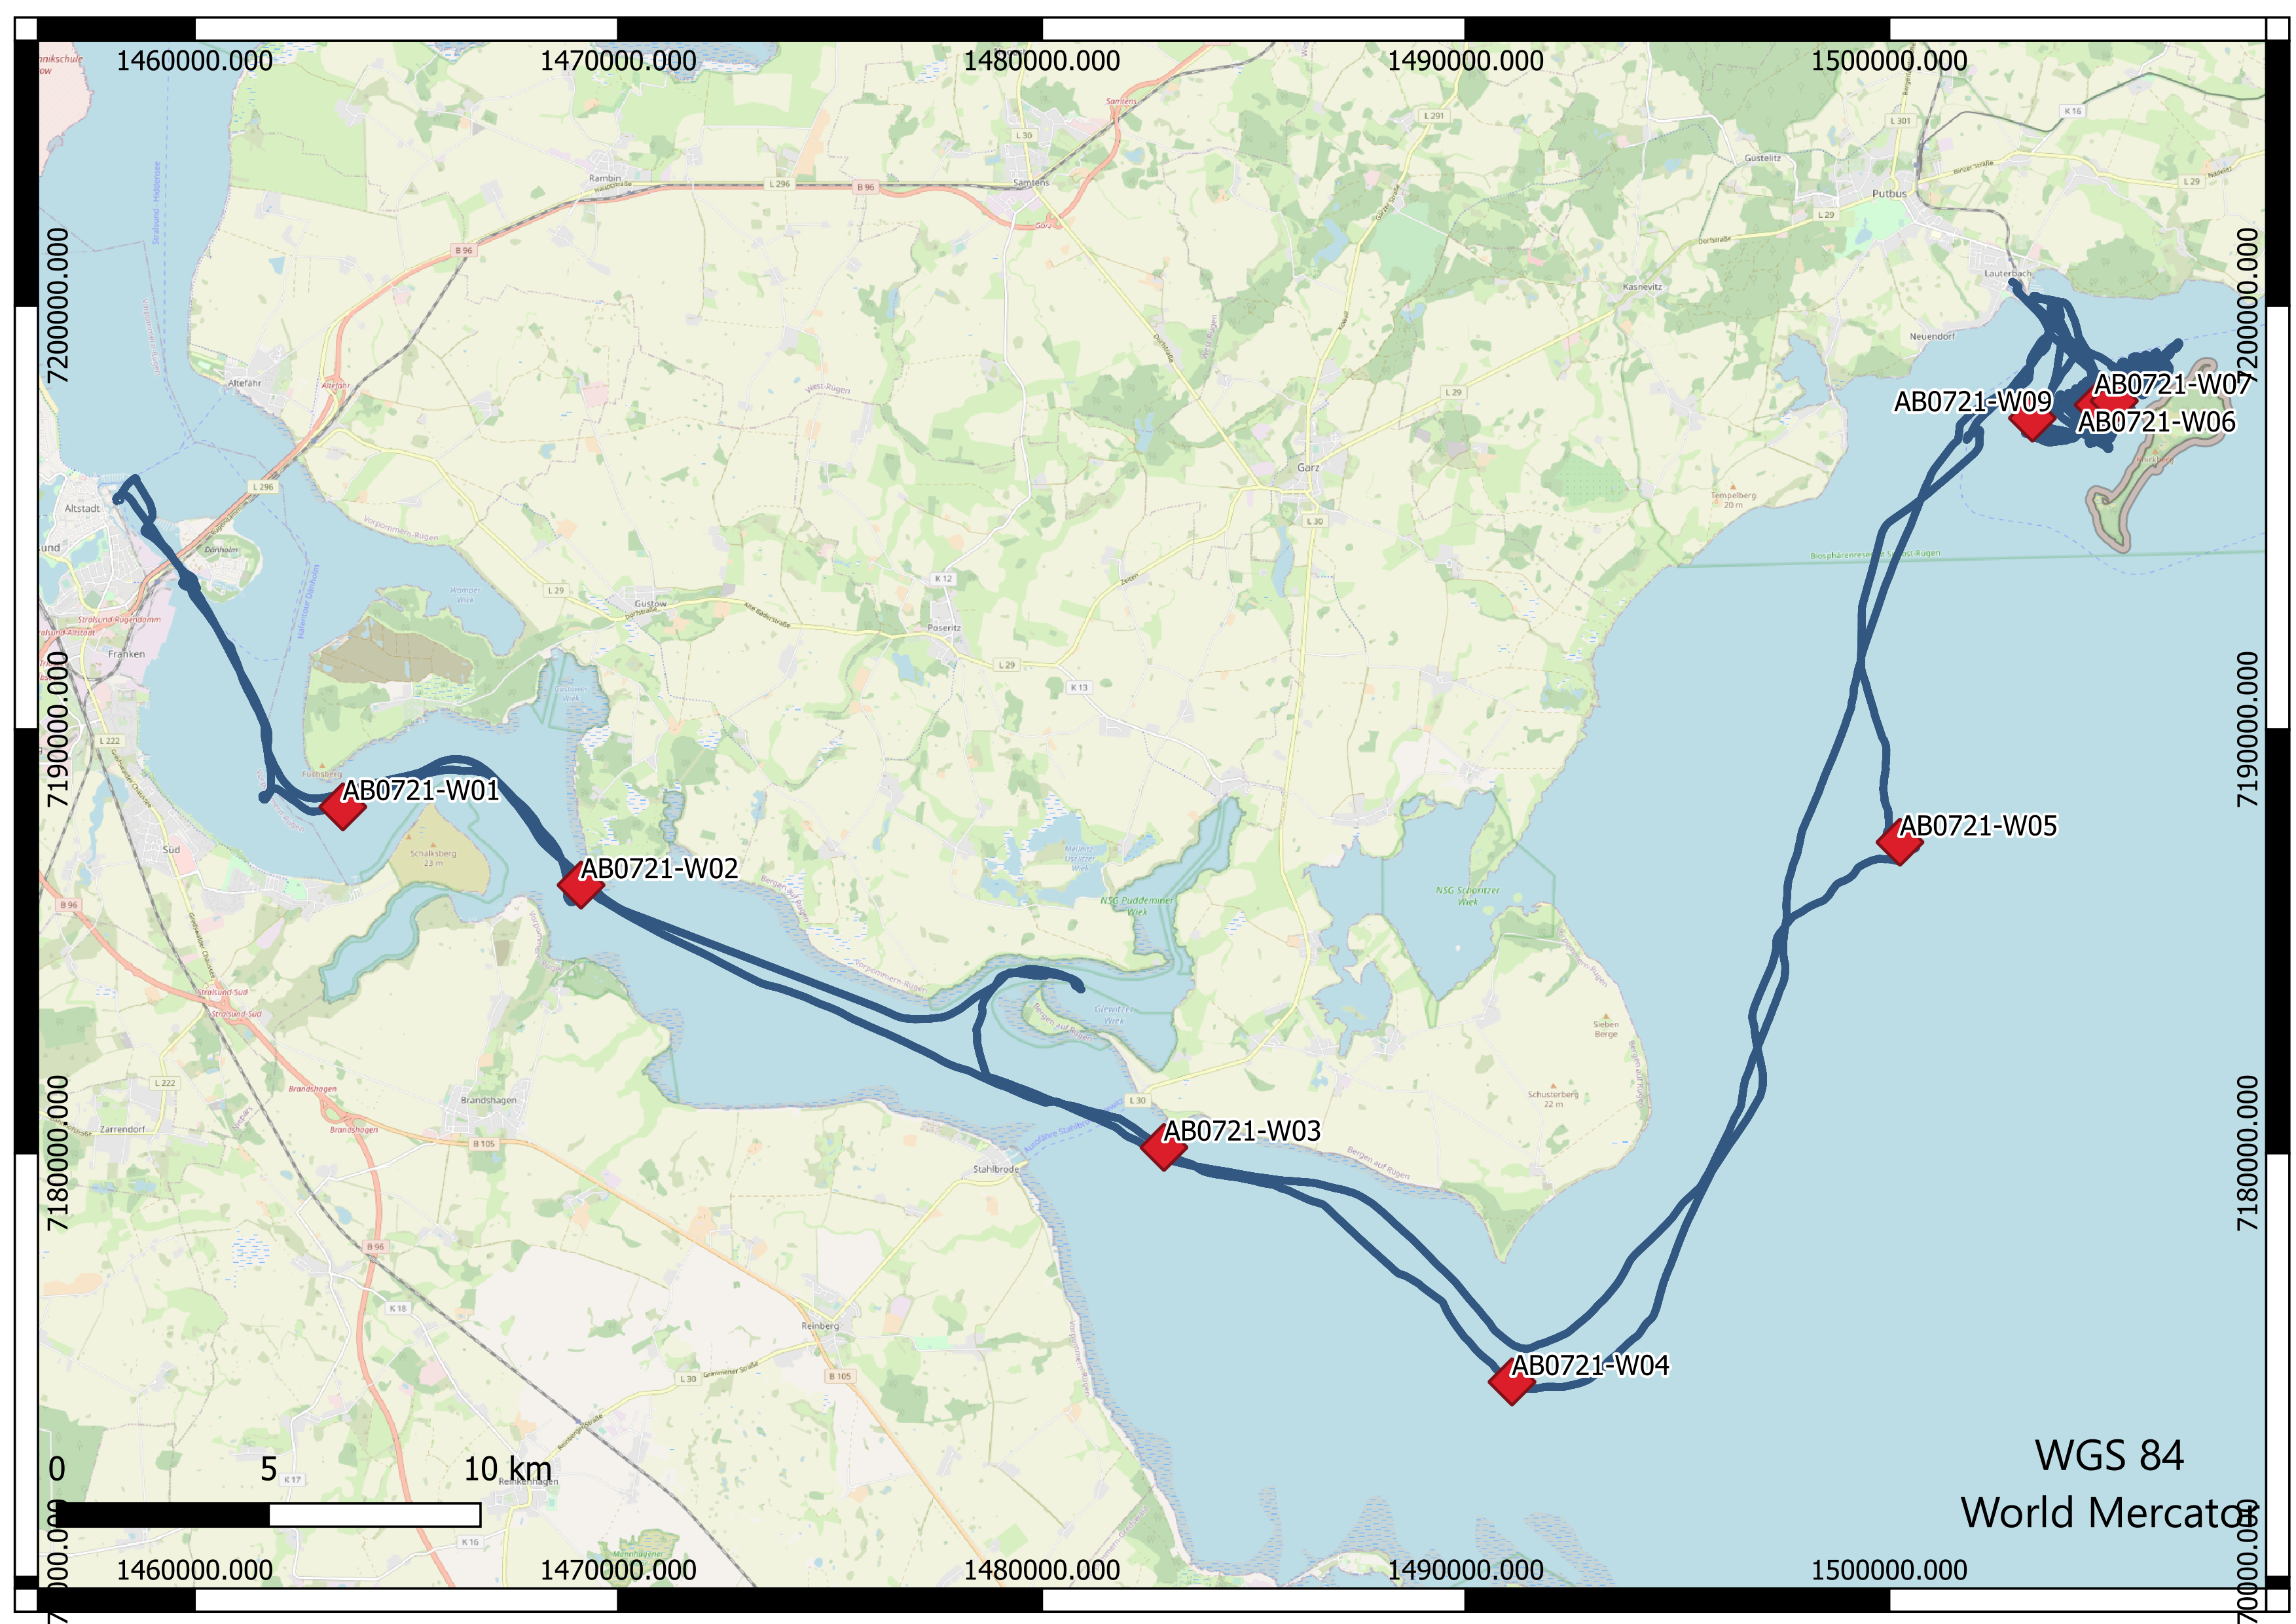
\includegraphics[width=0.8\linewidth]{Bilder/QGIS/Gesamte_route.png}
    \caption{Gesamte Route}
    \label{fig:route}
\end{figure}
\begin{figure}[]
    \centering
    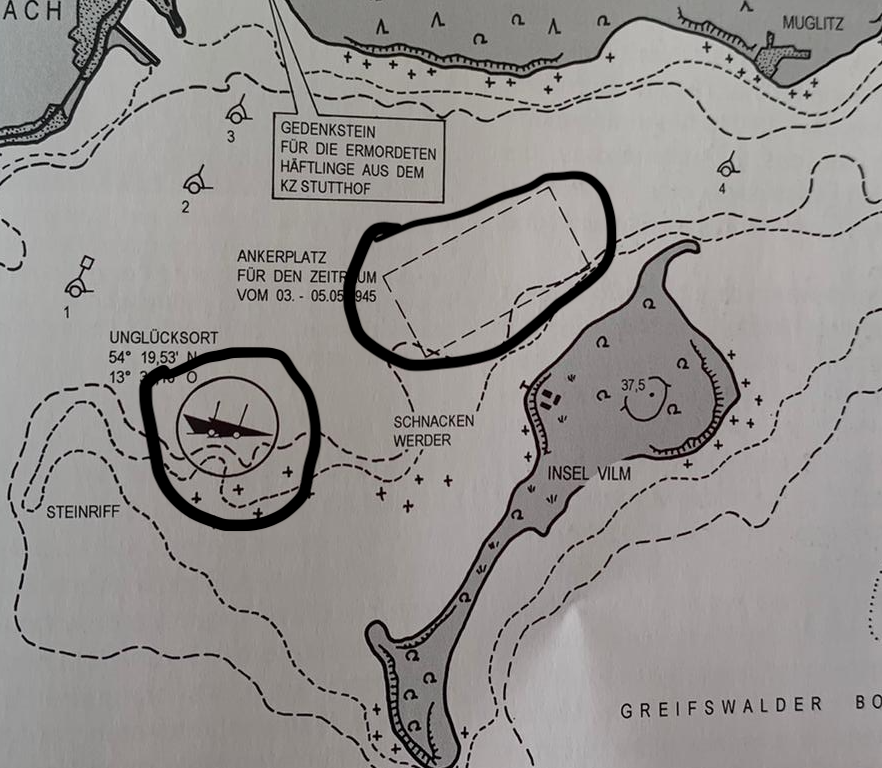
\includegraphics[width=0.8\linewidth]{Bilder/ungl.png}
    \caption{Dokumentierte Anker und Unglückstelle der Sprengstoffschuten.\cite{schiffsschicksale}}
    \label{fig:unglueck}
\end{figure}
\begin{figure}
    \centering
    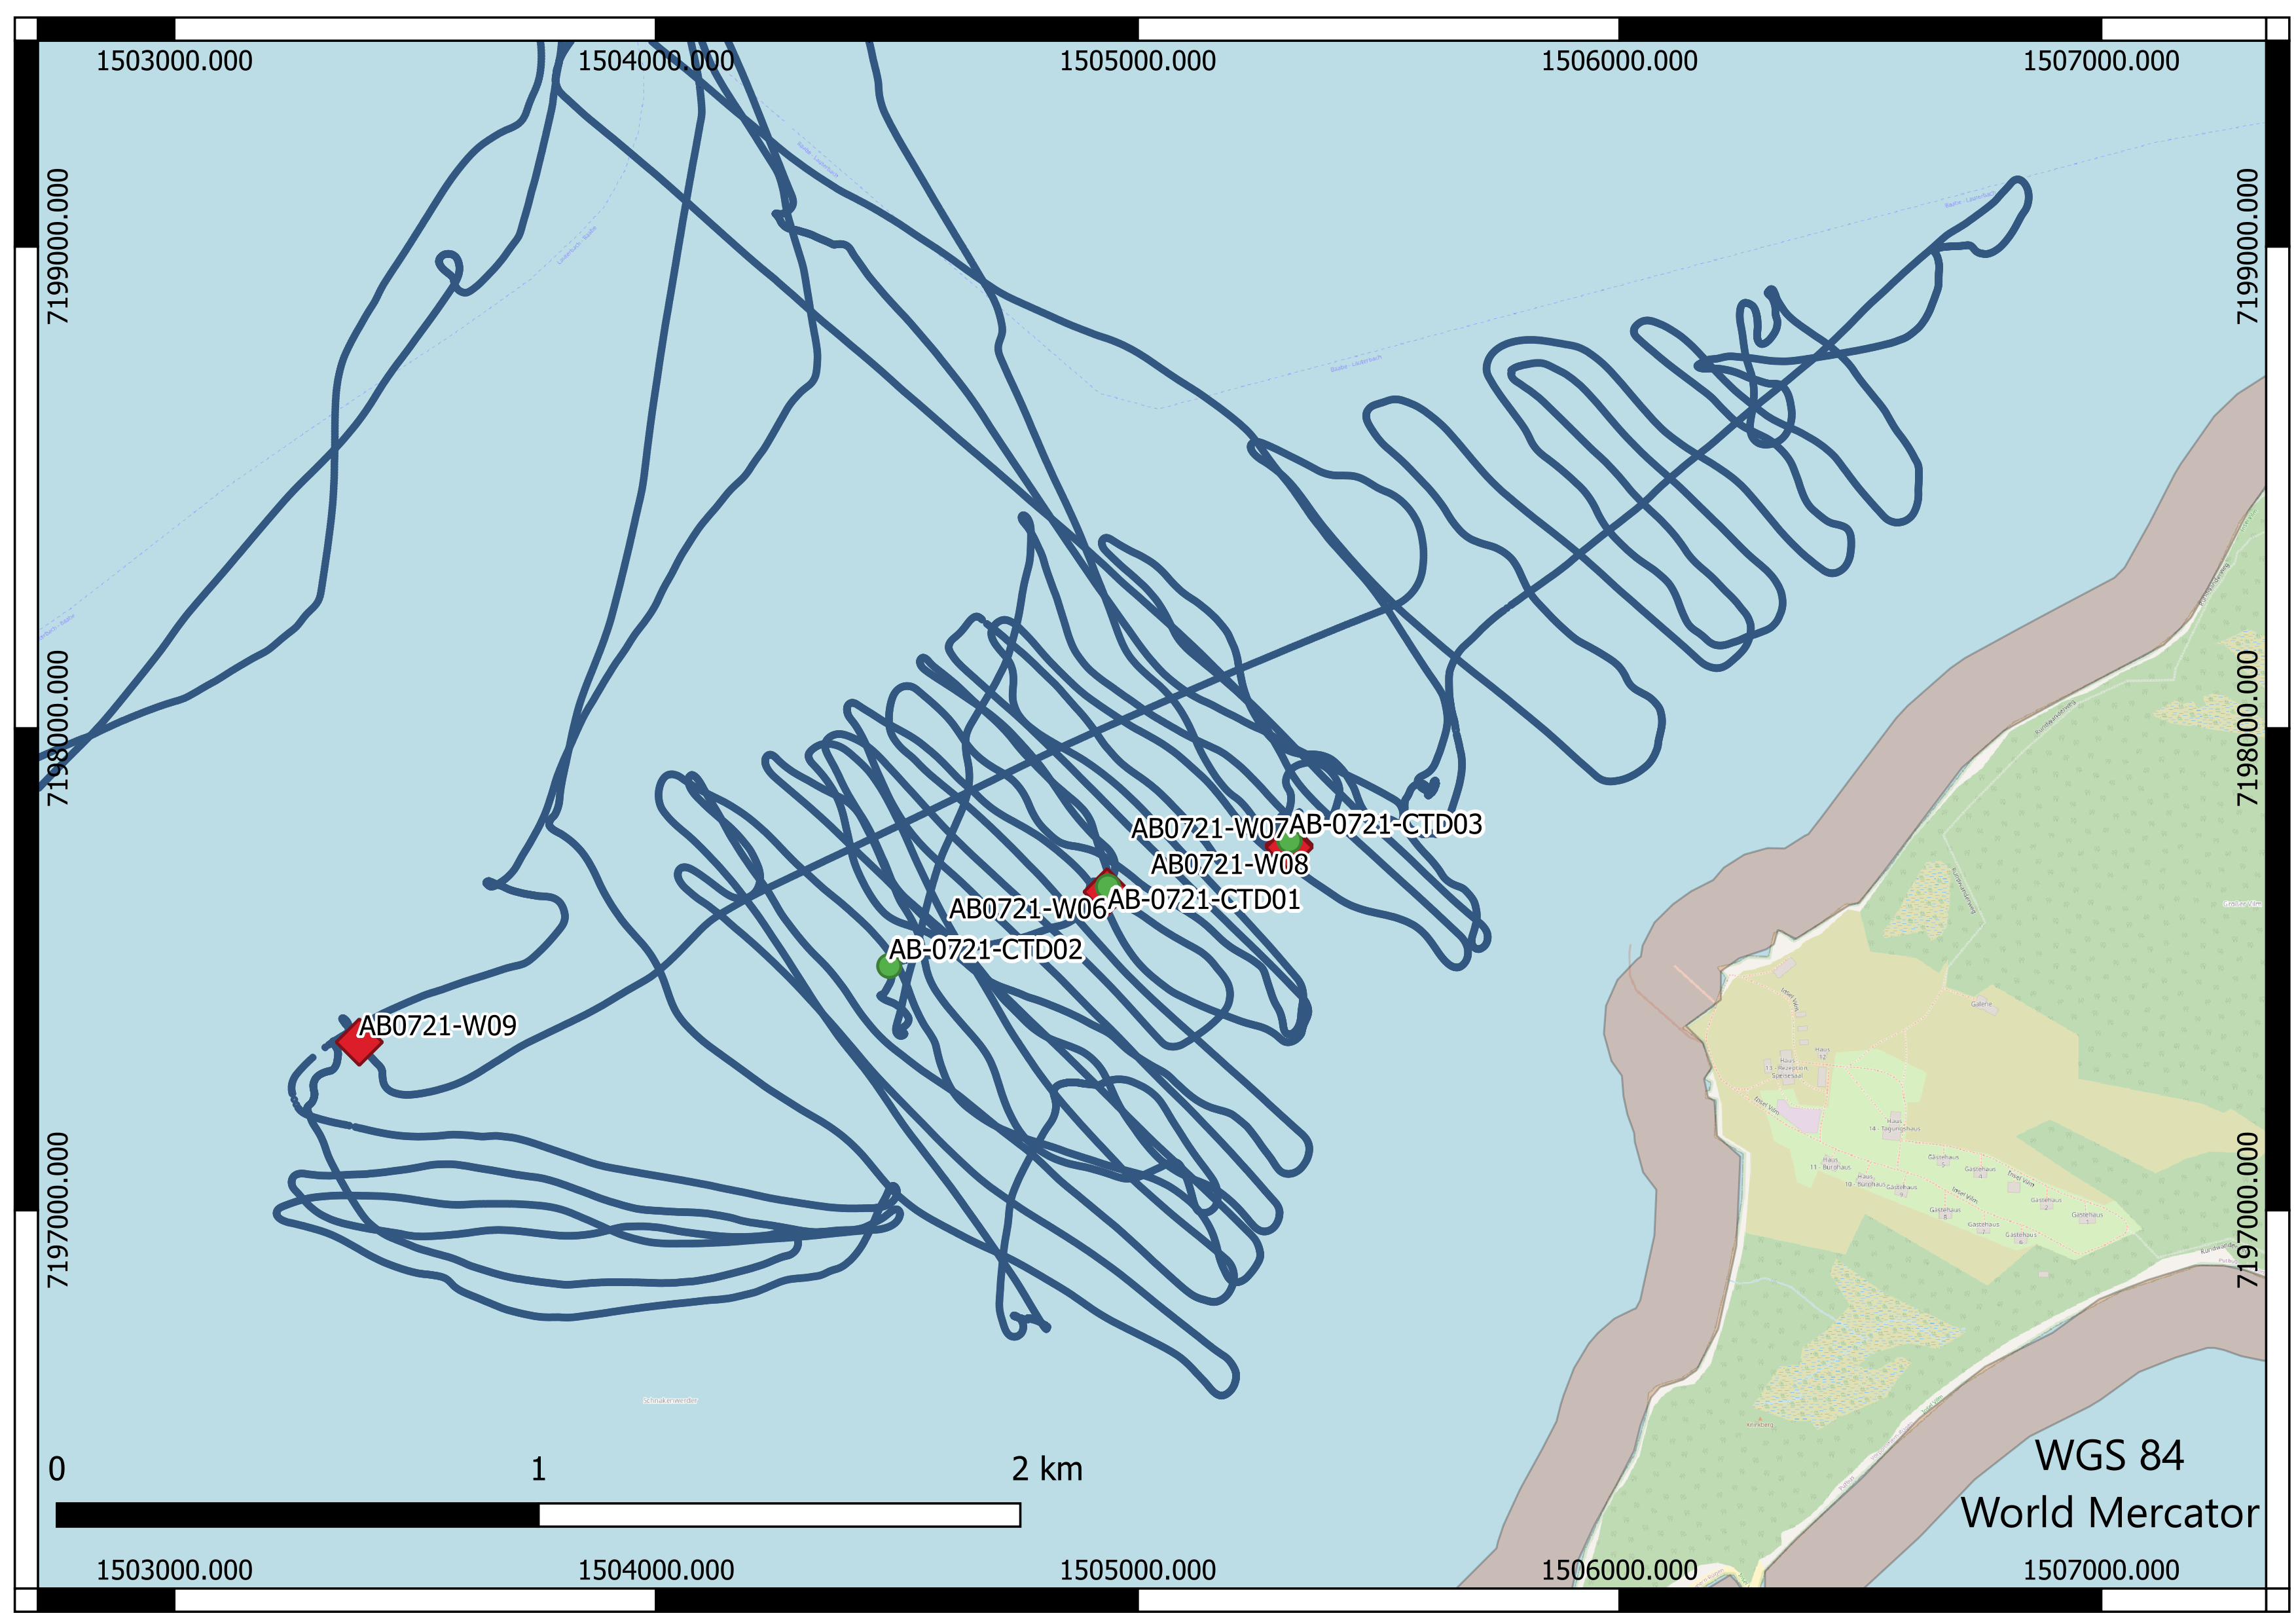
\includegraphics[width=0.8\linewidth]{Bilder/QGIS/multibeam.png}
    \caption{Multibeamfahrten. Wasserproben- und CTD-Stellen sind\\jeweils rot und grün markiert.}
    \label{fig:multibeam_route}
\end{figure}

    
\subsection{Wasserproben}
Hier muss noch was rein
\subsection{Sedimentproben}
Hier muss noch was rein
\subsection{Multiparametermessungen}

\subsection{ROV-Kartierungen}
\section{Ergebnisse}
\section{Diskussion der Ergebnisse}


% Activate the following line by filling in the right side. If for example the name of the root file is Main.tex, write
% "...root = Main.tex" if the chapter file is in the same directory, and "...root = ../Main.tex" if the chapter is in a subdirectory.
 
%!TEX root = TNTinderSee.tex 

\chapter[Fazit]{Fazit}





% Activate the following line by filling in the right side. If for example the name of the root file is Main.tex, write
% "...root = Main.tex" if the chapter file is in the same directory, and "...root = ../Main.tex" if the chapter is in a subdirectory.
 
%!TEX root =  TNTinderSee.tex

\chapter[Danksagungen]{Danksagungen}
Wir danken Prof Dr. Jens Greinert vom GEOMAR Kiel und Leiter der Arbeitsgruppe DeepSea-Monitoring. Er ist einfach der beste Wissenschaftspate, den wir uns hätten wünschen können.\\


Frank Schweikert und Dr. Hannes Imhof von der deutschen Meeresstiftung, für die tollen Tage und all die Hilfe an Board der Aldebaran. \\


Mareike Kampmeier vom GEOMAR Kiel für die geduldige Einführung am Multibeam und die vielen Erklärungen zum Thema Sprengstoffe im Wasser. \\


Dr. rer. nat. Inken Suck vom GEOMAR Kiel, der bestimmt coolsten ROV-Piloten dafür, dass sie uns gezeigt hat, wie man Unterwasserfahrzeuge richtig navigiert. \\


Maria Martinez Cabanas vom GEOMAR Kiel dafür, dass sie uns und unsere Proben in Ihre Labore mitgenommen hat, und geduldig stundenlang alle Fragen beantwortet hat.\\



Yifan Song vom GEOMAR Kiel dafür, dass er uns ganz praktisch beigebracht hat, wie man Videomaterial georeferenziert.

Besonders beeindruckt hat uns, dass uns die Wissenschaftler:innen wie selbstverständlich Samstag und Sonntag zur Seite standen und uns alles gezeigt haben.

Vielen Dank auch an Svenja Ehlers vom GEOMAR für ihre Hilfe und Geduld was das administrative der Reise anging und natürlich auch an Sofie Steinhausen von der deutschen Meeresstiftung, für die stets hilfsbereite Begleitung während des ganzen Wettbewerbes.


Dr. Kevin Köser vom GEOMAR Kiel für den inspirierenden Vortrag über Photogrammetrie \\


Yifan Song vom GEOMAR Kiel dafür, dass er uns ganz praktisch beigebracht hat, wie man Videomaterial georeferenziert.\\

Marek Czernohous für die insgesamt über 24 Stunden Fahrzeit, die Mate, Franzbrötchen und enorme Hilfe beim \LaTeX -Satz.\\



\bibliography{bibliography}
\bibliographystyle{plain}
% Activate the following line by filling in the right side. If for example the name of the root file is Main.tex, write
% "...root = Main.tex" if the chapter file is in the same directory, and "...root = ../Main.tex" if the chapter is in a subdirectory.
 
%!TEX root =  TNTinderSee.tex

\chapter[Anhang]{Anhang}




\end{document}